\documentclass[]{article}
\usepackage[utf8]{inputenc}
\usepackage[usenames,dvipsnames]{xcolor}
\usepackage{fullpage}
\usepackage[upright]{fourier}
\usepackage{tkz-graph}
\usetikzlibrary{arrows}
\thispagestyle{empty}
\begin{document}
\SetVertexNormal[Shape      = circle,
                 FillColor  = orange,
                 LineWidth  = 2pt]
\SetUpEdge[lw         = 1.5pt,
           color      = black,
           labelcolor = white,
           labeltext  = red,
           labelstyle = {sloped,draw,text=blue}]
\begin{center}
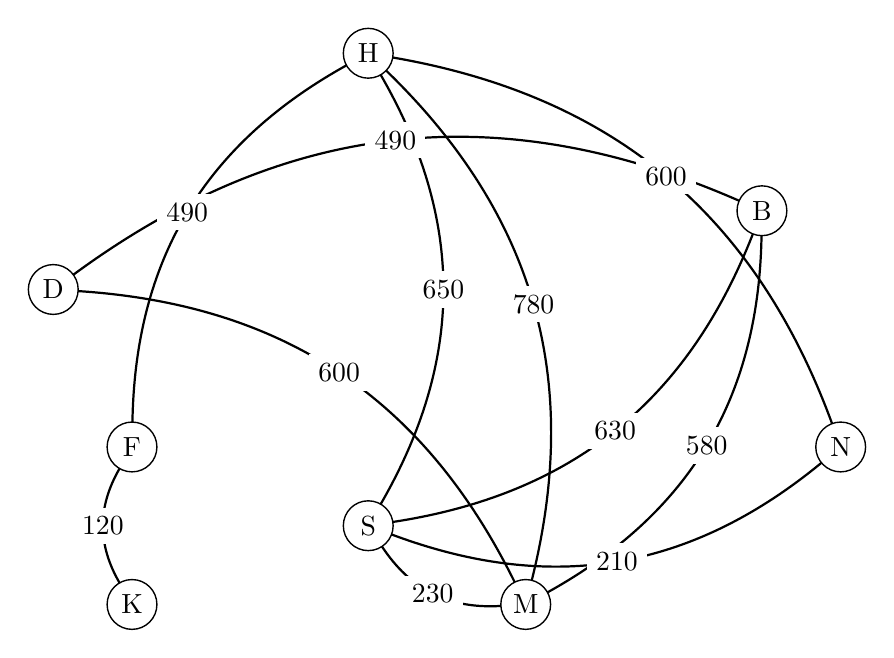
\begin{tikzpicture}
   \Vertex[x=0 ,y=0]{K}
   \Vertex[x=0 ,y=2]{F}
   \Vertex[x=-1,y=4]{D}
   \Vertex[x=3 ,y=7]{H}
   \Vertex[x=8 ,y=5]{B}
   \Vertex[x=9 ,y=2]{N}
   \Vertex[x=5 ,y=0]{M}
   \Vertex[x=3 ,y=1]{S}
   \tikzset{EdgeStyle/.append style = {bend left}}
   \Edge[label = $120$](K)(F)
   \Edge[label = $650$](H)(S)
   \Edge[label = $780$](H)(M)
   \Edge[label = $490$](D)(B)
   \Edge[label = $600$](D)(M)
   \Edge[label = $580$](B)(M)
   \Edge[label = $600$](H)(N)
   \Edge[label = $490$](F)(H)
   \tikzset{EdgeStyle/.append style = {bend right}}
   \Edge[label = $630$](S)(B)
   \Edge[label = $210$](S)(N)
   \Edge[label = $230$](S)(M)
\end{tikzpicture}
\end{center}

\end{document} 
